\documentclass[11pt,border=5pt]{standalone}
\usepackage{fontspec}
\setmainfont{cmunrm.otf}[BoldFont=cmunbx.otf,ItalicFont=cmunti.otf,BoldItalicFont=cmunbi.otf]
\usepackage{amsmath}
\usepackage{unicode-math}
\setmathfont{NewCMMath-Regular.otf}
\usepackage{tikz}
\usetikzlibrary{arrows.meta,patterns,angles,quotes}
\begin{document}
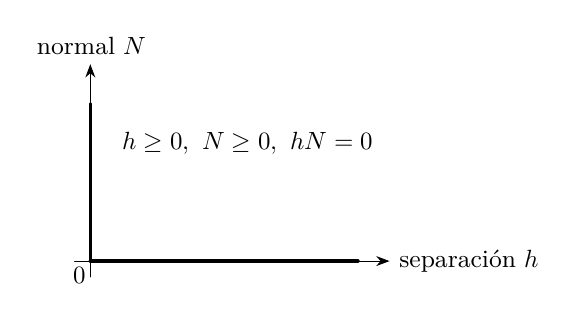
\begin{tikzpicture}[>=Stealth,font=\small,line cap=round,line join=round]
\draw[->,thin] (-0.2,0) -- (3.8,0) node[right] {separación $h$};
\draw[->,thin] (0,-0.2) -- (0,2.5) node[above] {normal $N$};
\node at (-0.14,-0.18) {$0$};
\draw[very thick] (0,0) -- (0,2);
\draw[very thick] (0,0) -- (3.4,0);
\node at (2,1.5) {$h\ge0,\ N\ge0,\ hN=0$};

\end{tikzpicture}
\end{document}
